\documentclass[10pt]{article}

\usepackage{amsmath, amsfonts, amsthm, fullpage, tikz, wrapfig, enumerate}

\newcommand{\card}[1]{\left| #1 \right|}
\newcommand{\nat}{\mathbb{N}}
\newcommand{\ints}{\mathbb{Z}}
\newcommand{\reals}{\mathbb{R}}
\newcommand{\chtitle}[1]{\noindent \vspace{5mm}\textbf{Chapter #1}\vspace{3mm}}
\newcommand{\images}{/home/gparker/classes/341/images}

\begin{document}
\begin{flushleft}
\noindent
\textbf{\noindent
Geoffrey Parker\\
CS 341 Automata Theory \\
Homework 4 \\
Due Tuesday, February 7}\\
\end{flushleft}
\noindent
This assignment covers Sections 5.9 - 5.11 and Chapter 6 \\

\noindent
\textbf{Sections 5.9 - 5.11}
\begin{enumerate}[1)]
\addtocounter{enumi}{14}
% ---
% 15
% ---

\item
Consider the problem of counting the number of words in a text file that may contain letters plus any  of the following characters:
\[<blank>\ <linefeed>\ <end-of-file>\ ,\ .\ ;\ :\ ?\ !\]
Define a word to be a string of letters that is preceded by either the beginning of the file or some non-letter character and that is followed by some non-letter character.  For example, there are 11 words in the following text:
\begin{flushleft}

\parindent 2cm

\texttt{\noindent
\hspace{2cm}The $<blank>$ $<blank>$ cat $<blank>$ $<linefeed>$\\
saw $<blank>$ the $<blank>$ $<blank>$ $<blank>$ rat $<linefeed>$\\
$<blank>$ with\\
$<linefeed>$ a $<blank>$ hat $<linefeed>$\\
on $<blank>$ the $<blank>$ $<blank>$ mat $<end-of-file>$
}
\end{flushleft}
Describe a very simple finite-state transducer that reads the characters in the file one at a time and solves the word counting problem.  Assume that there exists an output symbol with the property that, every time it is generated, an 
external counter gets incremented.

\begin{proof}[Solution]
If we assume $\#$ to be the counter character, this transducer will work:
\begin{center}
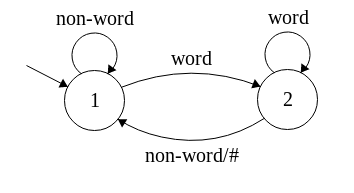
\includegraphics[scale=.4]{\images /hw4fst5_15solution.png}
\end{center}
\end{proof}

\pagebreak
\addtocounter{enumi}{1}
% ---
% 17
% ---

\item
Real bar code systems are more complex than the one we sketched in the book.  They 
must be able to encode all ten digits, for example.  There are several industry-standard 
formats for bar codes, including the common UPC code found on nearly everything we 
buy.  Search the web.  Find the encoding scheme used for UPC codes.  Describe a finite 
state transducer that reads the bars and outputs the corresponding decimal number.  You do 
not need to write out every state.  Show some at the beginning.  Then describe, in English, 
the structure of the rest of the machine.

\begin{center}
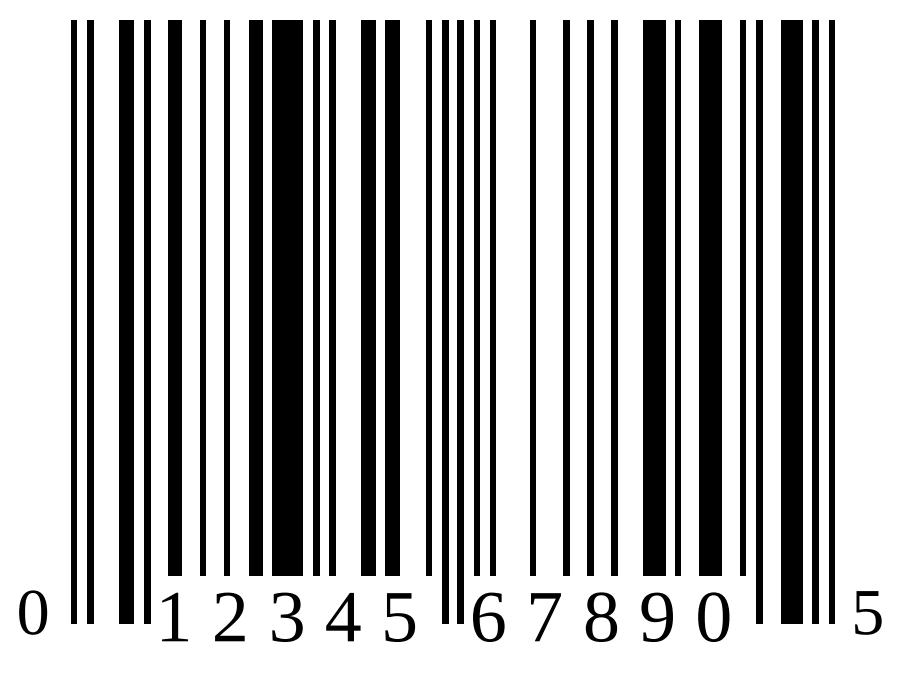
\includegraphics[scale=.1]{\images /hw4barcode.png}
\end{center}

\begin{proof}[Solution]
This is the start of a transducer which recognizes the start of a UPC code and outputs $S$, then processes the first 2 bars of the first number.\\
\begin{center}
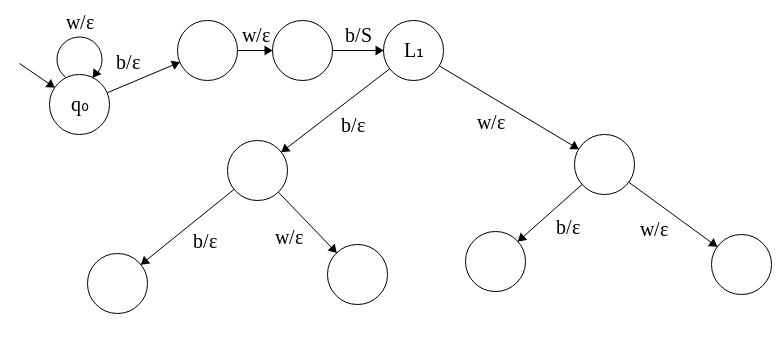
\includegraphics[scale=.4]{\images /hw4fst17solution.png}
\end{center}
From $L_1$, we begin to branch out into a binary tree representing all the possible sequences of white and black bars.  When we have read 7 bars, the patterns that represent the numbers 0-9 will all go to a state $L_2$ while outputing their respective number.  All other branches will go to a dead state and output nothing.  This will be repeated a total of 10 times, reading the left half of the barcode.  Then there will be a sequence similar to the $q_0$ to $L_1$ sequence to recognize the middle pattern, and then another 10 repeats of the digit transducer to recognize the right digits.  This is followed by a sequence to recognize the end, identical to the sequence to recognize the start, and you're done.
\end{proof}

\pagebreak
% ---
% 18
% ---

\item
Extend the description of the Soundex FSM that was started in Example 5.33 so that it can assign a code to the name Pfifer.  Remember that you must take into account the fact that every Soundex code is made up of exactly four characters.

\begin{proof}[Solution]
This transducer is by no means complete, but it should produce the correct output for Pfifer.
\begin{center}
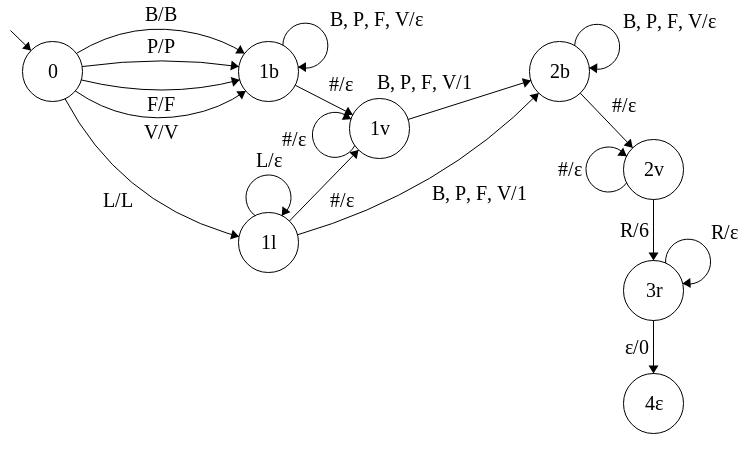
\includegraphics[scale=.4]{\images /hw4fsm18solution.png}
\end{center}
\end{proof}

% ---
% 19
% ---

\item
* Consider the weather/passport HMM of Example 5.37.  Trace the execution of the Viterbi and forward algorithms to answer the following questions:

\begin{enumerate}[a)]
%a
\item
Suppose that the report $\#\#\#L$ is received from Athens.  What was the most likely weather during the time of the report?

\begin{proof}[Solution]
\end{proof}
 
%b
\item
Is it more likely that $\#\#\#L$ came from London or from Athens?
\begin{proof}[Solution]
\end{proof}
\end{enumerate}

\addtocounter{enumi}{2}
% --
% 22
% --

\item
In I.1.2, we describe the Alternating Bit Protocol for handling message transmission in a network.  Use the FSM that describes the sender to answer the question, ``Is there any upper bound on the number of times a message may be retransmitted?''
\begin{proof}[Solution]
No.  There's a loop from $need ACK_1$ to $timed\ out_1$ that can be traversed infinitely, retransmitting the message each time.
\end{proof}

\end{enumerate}

\pagebreak
\textbf{Chapter 6}

\begin{enumerate}[1)]
% ---
% 1
% ---

\item
Describe in English, as briefly as possible, the language defined by each of these regular expressions:
\begin{enumerate}[a)]
%a
\item
$(b \cup ba) (b \cup a)^* (ab \cup b)$.
\begin{proof}[Solution]
The language of strings of $a$'s and $b$'s that are at least two characters long and begin and end with $b$.
\end{proof}

\end{enumerate}

% ---
% 2
% ---

\item
Write a regular expression to describe each of the following languages:
\begin{enumerate}[a)]
\addtocounter{enumii}{1}
%b
\item
$\{w \in \{a, b\}^*$ : $w$ does not end in $ba\}$.
\begin{proof}[Solution]
$(\epsilon \cup a \cup ((a \cup b)^*(aa \cup b))) $
\end{proof}

\addtocounter{enumii}{1}
%d
\item
$\{w \in \{0, 1\}^*$ : $w$ corresponds to the binary encoding, without leading $0$'s, of natural numbers that are evenly divisible by $4\}$.
\begin{proof}[Solution]
$0 \cup (1(0 \cup 1)^* 00)$
\end{proof}
%e
\item
$\{w \in \{0, 1\}^*$ : $w$ corresponds to the binary encoding, without leading $0$'s, of natural numbers that are powers of $4\}$.
\begin{proof}[Solution]
$0 \cup (1(00)^*)$
\end{proof}
\addtocounter{enumii}{2}
%h
\item
$\{w \in \{0, 1\}^*$ : $w$ does not have \texttt{001} as a substring\}.
\begin{proof}[Solution]
$(01 \cup 1)^*0^*$
\end{proof}
\addtocounter{enumii}{7}
%p
\item
* $\{w \in \{0, 1\}^*$ : $w$ contains exactly two occurrences of the substring \texttt{aa}\}.
\begin{proof}[Solution]
$(ab \cup b)^*aa(bab \cup b)^*aa(ba \cup b)^*$
\end{proof}
%q
\item
* $\{w \in \{a, b\}^*$ : $w$ contains no more than two occurrences of the substring \texttt{aa}\}.
\begin{proof}[Solution]
\end{proof}
\end{enumerate}

% ---
% 3
% ---
\item
Simplify each of the following regular expressions:
\begin{enumerate}[a)]
%a
\item
$(a \cup b)^* (a \cup \epsilon) b^*$.
\begin{proof}[Solution]
$(a \cup b)^* (a \cup \epsilon) b^* \equiv (a \cup b)^* b^* \equiv (a \cup b)^*$\\
\end{proof}
%b
\item
$(\emptyset ^* \cup b) b^*$.
\begin{proof}[Solution]
$(\emptyset ^* \cup b) b^* \equiv (\epsilon \cup b)b^* \equiv b^*$
\end{proof}
%c
\item
* $(a \cup b)^*a^* \cup b$.
\begin{proof}[Solution]
$(a \cup b)^*a^* \cup b \equiv (a \cup b)^* \cup b \equiv (a \cup b)^*$
\end{proof}
%d
\item
* $((a \cup b)^*)^*$.
\begin{proof}[Solution]
$((a \cup b)^*)^* \equiv (a \cup b)^*$
\end{proof}

\pagebreak
%e
\item
$((a \cup b)^+)^*$.
\begin{proof}[Solution]
$((a \cup b)^+)^* \equiv ((a \cup b)(a \cup b)^*)^* \equiv (a \cup b)^*(a \cup b)^* \equiv (a \cup b)^*$
\end{proof}
%f
\item
$a ( (a \cup b)(b \cup a) )^* \cup a ( (a \cup b) a )^* \cup a ( (b \cup a) b )^*$.
\begin{proof}[Solution]
$a ( (a \cup b)(a \cup b) )^*$
\end{proof}
\end{enumerate}
% ---
% 4
% ---
\item
For each of the following expressions $E$, answer the following three questions and prove your answer:
\begin{center}
\begin{enumerate}[(i)]
%i
\item
Is $E$ a regular expression?

%ii
\item
If $E$ is a regular expression, give a simpler regular expression.

%iii
\item
Does $E$ describe a regular language?
\end{enumerate}
\end{center}

\begin{enumerate}[a)]
\addtocounter{enumii}{1}
%b
\item
$(a^+a^nb^n)$.
\begin{proof}[Answer] $ $\\
\begin{enumerate}[(i)]
\item
No
\item
NA
\item
No
\end{enumerate}
\end{proof}
\begin{proof}
Regular expressions have no meaning for superscript $n$.
\end{proof}
\addtocounter{enumii}{1}
%d
\item
$(((ab) \cup c)^* \cap (b \cup c^*))$.
\begin{proof}[Answer] $ $\\
\begin{enumerate}[(i)]
\item
No
\item
NA
\item
Yes
\end{enumerate}
\end{proof}
\begin{proof}
The character $\cap$ is not a part of the language of regular expressions.  However, $((ab) \cup c)^*$ and $(b \cup c^*))$ are both regular expressions, and as such describe languages, so the intersection is also a language.
\end{proof}
\end{enumerate}

\pagebreak
\addtocounter{enumi}{4}
% ---
% 9
% ---

\item
* Consider the following FSM $M$:
\begin{center}
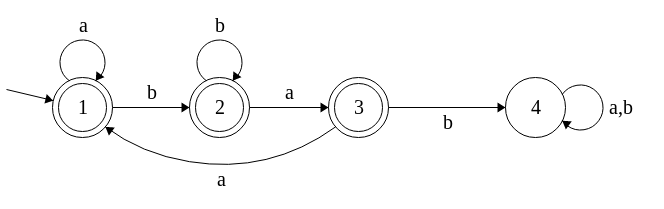
\includegraphics[scale=.45]{\images /hw4fsm9.png}
\end{center}

\begin{enumerate}[a)]
%a
\item
Show a regular expression for $L(M)$.
\begin{proof}[Solution]
\end{proof}
%b
\item
Describe $L(M)$ in English.
\begin{proof}[Solution]
\end{proof}
\end{enumerate}

\addtocounter{enumi}{5}
% ---
% 15
% ---
\item
Consider the following FSM M:

\begin{center}
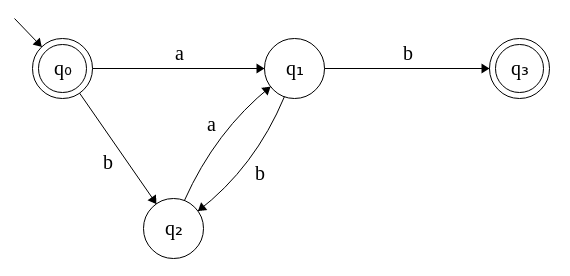
\includegraphics[scale=.45]{\images /hw4fsm15.png}
\end{center}

\begin{enumerate}[a)]
%a
\item
Show a regular expression for $L(M)$.
\begin{proof}[Solution]
$\epsilon \cup (a \cup b(ab)^*)b$
\end{proof}
%b
\item
Show a DFSM that accepts $\lnot L(M)$.
\begin{proof}[Solution]$ $\\
\begin{center}
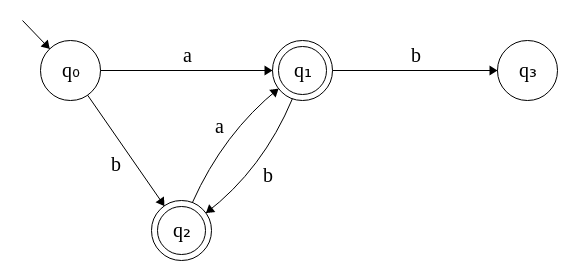
\includegraphics[scale=.4]{\images /hw4fsm15solution.png}
\end{center}
\end{proof}
\end{enumerate}

\addtocounter{enumi}{2}
% ---
% 18
% ---

\item
Let $\Sigma = \{a, b\}$.  Let $L = \{\epsilon, a, b\}$. Let $R$ be a relation defined on $\Sigma ^*$ as follows: $\forall xy\ (xRy$ iff $y = xb)$.  Let $R'$ be the reflexive, transitive closure of $R$.  Let $L' = \{x : \exists y \in L (yR'x)\}$.  Write a regular expression for $L'$.
\begin{proof}[Solution]
$(\epsilon \cup a \cup b)b*$
\end{proof}
\addtocounter{enumi}{1}
% ---
% 20
% ---
\item
For each of the following statements, state whether it is $True$ or $False$.  Prove your answer.
\begin{enumerate}[a)]
\addtocounter{enumii}{6}
%g
\item
If $\alpha$ and $\beta$ are any two regular expressions, then $(\alpha \cup \beta)^* = \alpha(\beta\alpha \cup \alpha)$.
\begin{proof}[Answer]
False.
\end{proof}
\begin{proof}
Let $\alpha = a$ and $\beta = b$.  Then $bbbb$ is an element of the language represented by $(\alpha \cup \beta)^*$, but not that of $\alpha(\beta\alpha \cup \alpha)$.
\end{proof}
%h
\item
If $\alpha$ and $\beta$ are any two regular expressions, then $(\alpha\beta)^*\alpha = \alpha(\beta\alpha)^*$.
\begin{proof}[Answer]
True.
\end{proof}
\begin{proof}
Let $r_1 = (\alpha\beta)^*\alpha$, and $r_2 = \alpha(\beta\alpha)^*$.  Let $k$ be then number of concatentations pulled from the kleene star.  Then if $k = 0$, $r_1 = \alpha$ and $r_2 = \alpha$.  If $k = 1$, $r_1 = \alpha \beta \alpha$ and $r_2 = \alpha \beta \alpha$.  If $k = 2$, $r_1 = \alpha \beta \alpha \beta \alpha$ and $r_2 = \alpha \beta \alpha \beta \alpha$. For any $k$ it's the same, $r_1 = r_2$ because you're just adding $\alpha \beta$ to the middle. 
\end{proof}
\end{enumerate}
\end{enumerate}
\end{document}
